\chapter{Evaluation}
\label{chapter:evaluation}
  In the previous chapter we described how we implemented our solution namely the data model that we used, the description of the signaling protocol, how we performed stream recording, how we overlayed interactive content to video and lastly how we deployed our solution. 

  In this chapter we describe how we tested our solution, show and analyze the results in order to validate the contributions of this thesis.

\section{Tests Objectives}

  We have tested our solution with real users for a better understanding of their difficulties and what can be done in order to improve our solution's usability.

  We have also tested the performance of our solution by measuring the used resources. Those performance tests are crucial to ensure that our solution is in fact stable and users can use it timelessly without decreasing the quality of their experience. 


  \section {Performance Tests}

     In this section we describe performance test scenarios that we have applied and their respective results.


    \subsection{Tests Scenarios}


      In order to benchmark our system, we have implemented a small \emph{Python} script using \emph{psutil}\footnote{\url{https://github.com/giampaolo/psutil} (Accessed March 27, 2016)} that collects with a periodicity of one second; CPU, physical memory information relative to each running process and network usage relative to each interface. 

      We would like to collect network information relative to each process, which \emph{nethogs}\footnote{\url{https://raboof.github.io/nethogs/} (Accessed March 27, 2016)} provide but it could not capture the network usage of some processes. Although this would be useful for a deep analysis, we know which network interfaces are used to establish connections between processes as we show on table \ref{table:interfacemap}.

  \begin{table}[!htb]
\centering
\caption{Mapping of connections by network interface}
\label{table:interfacemap}
\begin{tabular}{|l|l|}
\hline
\multicolumn{1}{|c|}{\textbf{Interface}} & \multicolumn{1}{c|}{\textbf{Connection}}         \\ \hline
Loopback & Web Server $\leftrightarrow$ MongoDB  \\ \hline
Loopback & Web Server $\leftrightarrow$ Kurento Media Server  \\ \hline
Loopback & Kurento Media Server $\leftrightarrow$ Kurento Repository $\leftrightarrow$ MongoDB  \\ \hline
Ethernet & Web Server $\leftrightarrow$ Client\\ \hline
Ethernet & Kurento Media Server $\leftrightarrow$ Client\\ \hline
\end{tabular}
\end{table}


      The performance test scenario that we have defined consists on two phases, the first phase consists only on having users, with similar computer and network specifications, entering sequentially on the conference room, the second phase consists on the users leaving the conference room. Each event, joining and leaving, occurs with intervals of one minute in total of thirteen minutes (780 seconds).

  


\subsection{Test Results}
  
      We are presenting in this sections the results of our performance tests after implementing our solution.

      Every time a user shares its camera or its screen in the context of a conference room, its offered video is sent to the server and independently from watching an individual stream or the mixed version the server just sends a unique stream back to the user.

      From the media server prespective if there are $n$ clients connected each of them sending and receiving one stream, it is expected that server sends and receives also $n$ streams. By so we expect that the amount of network increases linearly as users join a conference room.

      Figure \ref{fig:test_full_features_net} confirms our expectations, each vertical yellow line represents each event, the first seven events are users entering the conference room the next ones represent users leaving the conversation. 
      


\begin{figure}[!htb]
  \begin{center}
    \begin{tikzpicture}
	\begin{axis}[
	    width=\textwidth,
	   	height=8cm,
	    title={Network usage},
	    xlabel={Time [seconds]},
	    ylabel={Transfer rate [mbps]},
	    xmin=-10, xmax=850,
	    ymin=0, ymax=25,
	    xtick={0,60,...,2000},
	    ytick={0,5,...,100},
	    extra x ticks={0,60,...,2000},
    	extra x tick labels={,,},
		extra tick style={
			grid=major,
			major grid style={yellow,thick,solid},
			tick label style={rotate=90,anchor=east}
		},
     legend cell align=left,
     legend style={legend pos=north west,font=\tiny},
	    ymajorgrids=true,
	    grid style=dashed,
	]
	
	\addplot[color=Blue] table[x expr=\thisrowno{0}-122,y expr=\thisrowno{1}*8/1000000] {stats/test_full_features/sent_eth0.dat};
	\addlegendentry{Sent(eth0)}

	\addplot[color=Red] table[x expr=\thisrowno{0}-122,y expr=\thisrowno{1}*8/1000000] {stats/test_full_features/recv_eth0.dat};
	\addlegendentry{Recv(eth0)}

	\addplot[color=Green] table[x expr=\thisrowno{0}-122,y expr=\thisrowno{1}*8/1000000] {stats/test_full_features/recv_lo.dat};
	\addlegendentry{Sent/Recv(lo)}

	\end{axis}
\end{tikzpicture}


  \end{center}
  \caption{Network usage after implementing all features}
  \label{fig:test_full_features_net}
\end{figure}

      The blue peaks are caused by the signaling phase and web page downloads, including resources such as images, stylesheets and javascript files. 
      The green peaks are caused by that being transfered between \ac{KMS} and \emph{MongoDB} through \emph{Kurento Repository} each peak occurs each time a block of video is recorded which in this case is every ten seconds. 
      The recordings are synchronized so all user and mixed blocks starts and ends at the same time, that's why the amount of work done every ten seconds accumulates and because this is performed locally the maximum transfer rate is limited by the performance of the memory as buffers are written to buffers then to disks. 
      Client's sent data transfer rate has no significant peaks as signaling information contains few information.

      Figure \ref{fig:summary_full_net} shows the average transmission rate per interval of consecutive events. 

\begin{figure}[!htb]
  \begin{center}
    \begin{tikzpicture}
	\begin{axis}[
	    width=\textwidth,
	   	height=8cm,
	    title={Network usage},
	    xlabel={Time [seconds]},
	    ylabel={Transfer rate [mbps]},
	    xmin=-10, xmax=850,
	    ymin=0, ymax=10,
	    xtick={0,60,...,2000},
	    ytick={0,1,...,100},
	    extra x ticks={0,60,...,2000},
    	extra x tick labels={,,},
		extra tick style={
			grid=major,
			major grid style={yellow,thick,solid},
			tick label style={rotate=90,anchor=east}
		},
     legend cell align=left,
     legend style={legend pos=north west,font=\tiny},
	    ymajorgrids=true,
	    grid style=dashed,
	]
	
	\addplot[color=Blue] table[x expr=\thisrowno{0}-122,y expr=\thisrowno{1}*8/1000000] {stats/test_full_features/summary_sent_eth0.dat};
	\addlegendentry{Sent(eth0)}

	\addplot[color=Red] table[x expr=\thisrowno{0}-122,y expr=\thisrowno{1}*8/1000000] {stats/test_full_features/summary_recv_eth0.dat};
	\addlegendentry{Recv(eth0)}

	\addplot[color=Green] table[x expr=\thisrowno{0}-122,y expr=\thisrowno{1}*8/1000000] {stats/test_full_features/summary_sent_lo.dat};
	\addlegendentry{Sent/Recv(lo)}

	\end{axis}
\end{tikzpicture}


  \end{center}
  \caption{Average network usage per interval of events after implementing all features}
  \label{fig:summary_full_net}
\end{figure}

If we consider all streams equal and an incoming stream uses $x$kbps, with $n$ incoming streams the rate of data received at \ac{KMS} is $nx$ and the expected rate of data transfered to \emph{Kurento Repo} using localhost is $(n+1)x$. Due to the data being transfered also from \emph{Kurento Repo} to \emph{MongoDB} via localhost, the expected total rate of data transfered through localhost is $2((n+1)x) = (2n+2)x$, which explains the reason for the average amount of data transfered through localhost being more than twice the average amount of data received from users.

With this results we conclude that if we want to scale our solution's storage using the \emph{MongoDB}'s cluster configuration, both \emph{Kurento Repository} and \emph{MongoDB} should be installed in the same machine because the loopback interface can handle bigger transfer rates than the remaining network interfaces. For the same reason another possible configuration for scaling the storage is to install both \emph{Kurento Repository} and \ac{KMS} on the same machine.

Figure \ref{fig:test_full_features_mem} shows the memory usage during our performance test case. Both \ac{JVM}, \emph{MongoDB} and \ac{KMS} performs their own memory management by holding and recycling objects when needed. The expected and observed behavior of the memory usage is growth memory usage while the users are entering in the conference room and a memory usage stabilization afterwards.


\begin{figure}[!htb]
  \begin{center}
    \begin{tikzpicture}
	\begin{axis}[
	    width=\textwidth,
	   	height=8cm,
	    title={Memory Usage},
	    xlabel={Time [seconds]},
	    ylabel={Memory [MB]},
	    xmin=-10, xmax=850,
	    ymin=0, ymax=1800,
	    xtick={0,60,...,2000},
	    ytick={0,200,...,2000},
	    extra x ticks={0,60,...,2000},
    	extra x tick labels={,,},
		extra tick style={
			grid=major,
			major grid style={yellow,thick,solid},
			tick label style={rotate=90,anchor=east}
		},
     legend cell align=left,
     legend style={legend pos=north west,font=\tiny},
	    ymajorgrids=true,
	    grid style=dashed,
	] 

		\addplot[smooth,color=Blue] table[x expr=\thisrowno{0}-122,y expr=\thisrowno{1}/1000000] {stats/test_full_features/res_7_mongod.dat};
		\addlegendentry{Mongod}

		\addplot[smooth,color=Red] table[x expr=\thisrowno{0}-122,y expr=\thisrowno{1}/1000000] {stats/test_full_features/res_67_kurento-media-server.dat};
		\addlegendentry{Kurento Media Server}

		\addplot[smooth,color=Green] table[x expr=\thisrowno{0}-122,y expr=\thisrowno{1}/1000000] {stats/test_full_features/res_35_kurento-repo.dat};
		\addlegendentry{Kurento Repository}

		\addplot[smooth,color=Magenta] table[x expr=\thisrowno{0}-122,y expr=\thisrowno{1}/1000000] {stats/test_full_features/res_233_bash.dat};
		\addlegendentry{Java}

	\end{axis}
\end{tikzpicture}



  \end{center}
  \caption{Memory usage after implementing all features}
  \label{fig:test_full_features_mem}
\end{figure}

\emph{MongoDB} memory usage keeps increasing because it tries to fit part of the database on \ac{RAM} for fast read access. \emph{MongoDB} checkpoints data to disk every 60 seconds or when journal data exceeds 2GB\footnote{\url{https://docs.mongodb.org/manual/faq/storage/}(Accessed March 28, 2016)}, that explains the small memory usage peaks during our test case. When the conference room is empty no there are no video recordings, which explains the memory stabilization at the end.

Figure \ref{fig:test_full_features_cpu} shows the percentage of \ac{CPU} usage during our performance test case. As we can see, the amount of \ac{CPU} increases and decreases linearly in function of the amount of conference participants. 

\begin{figure}[!htb]
  \begin{center}
    \begin{tikzpicture}
	\begin{axis}[
	    width=\textwidth,
	   	height=6cm,
	    title={CPU usage},
	    xlabel={Time [seconds]},
	    ylabel={CPU [percentage]},
	    xmin=-10, xmax=850,
	    ymin=0, ymax=1200,
	    xtick={0,60,...,2000},
	    ytick={0,200,...,2000},
	    extra x ticks={0,60,...,2000},
    	extra x tick labels={,,},
		extra tick style={
			grid=major,
			major grid style={yellow,thick,solid},
			tick label style={rotate=90,anchor=east}
		},
     legend cell align=left,
     legend style={legend pos=north west,font=\tiny},
	    ymajorgrids=true,
	    grid style=dashed,
	] 

		\addplot[smooth,color=Blue] table[x expr=\thisrowno{0}-122,y index=1] {stats/test_full_features/cpu_7_mongod.dat};
		\addlegendentry{Mongod}

		\addplot[smooth,color=Red] table[x expr=\thisrowno{0}-122,y index=1] {stats/test_full_features/cpu_67_kurento-media-server.dat};
		\addlegendentry{Kurento Media Server}

		\addplot[smooth,color=Green] table[x expr=\thisrowno{0}-122,y index=1] {stats/test_full_features/cpu_35_kurento-repo.dat};
		\addlegendentry{Kurento Repository}

		\addplot[smooth,color=Magenta] table[x expr=\thisrowno{0}-122,y index=1] {stats/test_full_features/cpu_233_bash.dat};
		\addlegendentry{Java}

	\end{axis}

\end{tikzpicture}


  \end{center}
  \caption{Percentage of CPU used during the performance tests}
  \label{fig:test_full_features_cpu}
\end{figure}

Figure \ref{fig:test_full_features_cpu_zoom} is the same as figure \ref{fig:test_full_features_cpu} but zoomed over \emph{MongoDB}, \emph{Java} and \emph{Kurento Repository}. As we can see there are periodic processing peaks every ten seconds that are due to block recording. 

\begin{figure}[!htb]
  \begin{center}
    \begin{tikzpicture}
	\begin{axis}[
	    width=\textwidth,
	   	height=6cm,
	    title={CPU usage},
	    xlabel={Time [seconds]},
	    ylabel={CPU [percentage]},
	    xmin=-10, xmax=850,
	    ymin=0, ymax=100,
	    xtick={0,60,...,2000},
	    ytick={0,20,...,2000},
	    extra x ticks={0,60,...,2000},
    	extra x tick labels={,,},
		extra tick style={
			grid=major,
			major grid style={yellow,thick,solid},
			tick label style={rotate=90,anchor=east}
		},
     legend cell align=left,
     legend style={legend pos=north west,font=\tiny},
	    ymajorgrids=true,
	    grid style=dashed,
	] 

		\addplot[smooth,color=blue] table[x expr=\thisrowno{0}-122,y index=1] {stats/test_full_features/cpu_7_mongod.csv};
		\addlegendentry{Mongod}

		\addplot[smooth,color=red] table[x expr=\thisrowno{0}-122,y index=1] {stats/test_full_features/cpu_67_kurento-media-server.csv};
		\addlegendentry{Kurento Media Server}

		\addplot[smooth,color=green] table[x expr=\thisrowno{0}-122,y index=1] {stats/test_full_features/cpu_35_kurento-repo.csv};
		\addlegendentry{Kurento Repository}

		\addplot[smooth,color=magenta] table[x expr=\thisrowno{0}-122,y index=1] {stats/test_full_features/cpu_233_bash.csv};
		\addlegendentry{Java}

	\end{axis}

\end{tikzpicture}


  \end{center}
  \caption{Percentage of CPU used during the performance tests}
  \label{fig:test_full_features_cpu_zoom}
\end{figure}

   Figure \ref{fig:summary_full_cpu} shows the average used \ac{CPU} per interval of consecutive events. 

\begin{figure}[!htb]
  \begin{center}
    \begin{tikzpicture}
	\begin{axis}[
	    width=\textwidth,
	   	height=6cm,
	    title={CPU usage},
	    xlabel={Time [seconds]},
	    ylabel={Transfer rate [kB/s]},
	    xmin=-10, xmax=850,
	    ymin=0, ymax=1400,
	    xtick={0,60,...,2000},
	    ytick={0,200,...,2000},
	    extra x ticks={0,60,...,2000},
    	extra x tick labels={,,},
		extra tick style={
			grid=major,
			major grid style={yellow,thick,solid},
			tick label style={rotate=90,anchor=east}
		},
     legend cell align=left,
     legend style={legend pos=north west,font=\tiny},
	    ymajorgrids=true,
	    grid style=dashed,
	]
	
		\addplot[color=Blue] table[x expr=\thisrowno{0}-122,y index=1] {stats/summary_full_cpu_mongo.csv};
		\addlegendentry{Mongod}

		\addplot[color=Red] table[x expr=\thisrowno{0}-122,y index=1] {stats/summary_full_cpu_kms.csv};
		\addlegendentry{Kurento Media Server}

		\addplot[color=Green] table[x expr=\thisrowno{0}-122,y index=1] {stats/summary_full_cpu_kr.csv};
		\addlegendentry{Kurento Repository}

		\addplot[color=Magenta] table[x expr=\thisrowno{0}-122,y index=1] {stats/summary_full_cpu_play.csv};
		\addlegendentry{Java}


	\end{axis}
\end{tikzpicture}


  \end{center}
  \caption{Average percentage of CPU used per interval of events after implementing all features (zoomed)}
  \label{fig:summary_full_cpu}
\end{figure}

  Just for testing purposes we have done the same performance tests without detecting \emph{QR codes} in order to understand how \ac{CPU} intensive is this task. Figure \ref{fig:test_without_qrcode_cpu} shows the results for the same experience but with \emph{QR code} detection disabled.

  \begin{figure}[!htb]
  \begin{center}
    \begin{tikzpicture}
	\begin{axis}[
	    width=\textwidth,
	   	height=6cm,
	    title={CPU usage},
	    xlabel={Time [seconds]},
	    ylabel={CPU [percentage]},
	    xmin=-10, xmax=850,
	    ymin=0, ymax=600,
	    xtick={0,100,...,2000},
	    ytick={0,100,...,2000},
	    extra x ticks={10,70,...,1000},
    	extra x tick labels={,,},
		extra tick style={
			grid=major,
			major grid style={yellow,thick,solid},
			tick label style={rotate=90,anchor=east}
		},
     legend cell align=left,
     legend style={legend pos=north west,font=\tiny},
	    ymajorgrids=true,
	    grid style=dashed,
	] 
	

		\addplot[smooth,color=Blue] table[x expr=\thisrowno{0}-35,y expr=\thisrowno{1}] {stats/test_without_qrcode/cpu_7_mongod.dat};
		\addlegendentry{Mongod}

		\addplot[smooth,color=Red] table[x expr=\thisrowno{0}-35,y expr=\thisrowno{1}] {stats/test_without_qrcode/cpu_67_kurento-media-server.dat};
		\addlegendentry{Kurento Media Server}

		\addplot[smooth,color=Green] table[x expr=\thisrowno{0}-35,y expr=\thisrowno{1}] {stats/test_without_qrcode/cpu_35_kurento-repo.dat};
		\addlegendentry{Kurento Repository}

		\addplot[smooth,color=Magenta] table[x expr=\thisrowno{0}-35,y expr=\thisrowno{1}] {stats/test_without_qrcode/cpu_233_bash.dat};
		\addlegendentry{Java}

	\end{axis}
\end{tikzpicture}


  \end{center}
  \caption{Percentage of CPU used during the performance tests without QR code detection}
  \label{fig:test_without_qrcode_cpu}
\end{figure}

We conclude that \emph{QR code} detection is a very intensive task, approximately doubling the amount of work performed by \ac{CPU}. Without this feature the network and memory usage had insignificant changes compared to \ac{CPU} usage.



  \begin{figure}[!htb]
  \begin{center}
    \begin{tikzpicture}
	\begin{axis}[
	    width=\textwidth,
	   	height=6cm,
	    title={CPU usage},
	    xlabel={Time [seconds]},
	    ylabel={CPU [percentage]},
	    xmin=-10, xmax=1690,
	    ymin=0, ymax=1200,
	    xtick={0,120,...,2000},
	    ytick={0,200,...,2000},
	    extra x ticks={0,60,...,2000},
    	extra x tick labels={,,},
		extra tick style={
			grid=major,
			major grid style={yellow,thick,solid},
			tick label style={rotate=90,anchor=east}
		},
     legend cell align=left,
     legend style={legend pos=north west,font=\tiny},
	    ymajorgrids=true,
	    grid style=dashed,
	] 

		\addplot[smooth,color=Blue] table[x expr=\thisrowno{0}-96,y index=1] {stats/test_two_times/cpu_7_mongod.dat};
		\addlegendentry{Mongod}

		\addplot[smooth,color=Red] table[x expr=\thisrowno{0}-96,y index=1] {stats/test_two_times/cpu_67_kurento-media-server.dat};
		\addlegendentry{Kurento Media Server}

		\addplot[smooth,color=Green] table[x expr=\thisrowno{0}-96,y index=1] {stats/test_two_times/cpu_35_kurento-repo.dat};
		\addlegendentry{Kurento Repository}

		\addplot[smooth,color=Magenta] table[x expr=\thisrowno{0}-96,y index=1] {stats/test_two_times/cpu_233_bash.dat};
		\addlegendentry{Java}

	\end{axis}

\end{tikzpicture}


  \end{center}
  \caption{Percentage of CPU used during two consecutive test cases}
  \label{fig:test_two_times_cpu}
\end{figure}


\begin{figure}[!htb]
  \begin{center}
    \begin{tikzpicture}
	\begin{axis}[
	    width=\textwidth,
	   	height=6cm,
	    title={Memory Usage},
	    xlabel={Time [seconds]},
	    ylabel={Memory [MB]},
	    xmin=-10, xmax=1690,
	    ymin=0, ymax=1800,
	    xtick={0,120,...,2000},
	    ytick={0,200,...,2000},
	    extra x ticks={0,60,...,2000},
    	extra x tick labels={,,},
		extra tick style={
			grid=major,
			major grid style={yellow,thick,solid},
			tick label style={rotate=90,anchor=east}
		},
     legend cell align=left,
     legend style={legend pos=north west,font=\tiny},
	    ymajorgrids=true,
	    grid style=dashed,
	] 

		\addplot[smooth,color=Blue] table[x expr=\thisrowno{0}-72,y expr=\thisrowno{1}/1000000] {stats/test_two_times3/res_7_mongod.dat};
		\addlegendentry{Mongod}

		\addplot[smooth,color=Red] table[x expr=\thisrowno{0}-72,y expr=\thisrowno{1}/1000000] {stats/test_two_times3/res_68_kurento-media-server.dat};
		\addlegendentry{Kurento Media Server}

		\addplot[smooth,color=Green] table[x expr=\thisrowno{0}-72,y expr=\thisrowno{1}/1000000] {stats/test_two_times3/res_35_kurento-repo.dat};
		\addlegendentry{Kurento Repository}

		\addplot[smooth,color=Magenta] table[x expr=\thisrowno{0}-72,y expr=\thisrowno{1}/1000000] {stats/test_two_times3/res_234_bash.dat};
		\addlegendentry{Java}

	\end{axis}
\end{tikzpicture}



  \end{center}
  \caption{Memory usage during two consecutive test cases}
  \label{fig:test_two_times_mem}
\end{figure}

\section {Usability Tests}
     In this section we describe usability test scenarios that we have applied and their respective results.


    \subsection{Tests Scenarios}

      In order to the usability of our solution, we haver performed usability tests with the help of real users with different backgrounds and ages.

      We handled a guide to the users with five tasks to perform, the metrics we used for each task were: number of clicks, number of errors including a description and time spent. 

      The tasks we asked to the user are:

      \begin{enumerate}
      \item Login into the system with the provided credentials and accept the received friendship request. Find the coordinator's brother and add him as a friend.

      \item Create a private conference room, enter and share your screen, add the coordinator to the conference room and chat with him. After that use the collaborative editor in order to write at the same time as the coordinator. Lastly save the editor and leave the conference room.

      \item Enter in the conference room correspondent to the third task as an observer and navigate to the specified annotation. Watch the video until a list of topics is overlayed in the video and choose one of them and leave the conference room.

      \item Enter in the conference room correspondent to the fourth task by sharing your camera and create a time annotation in the instant of time when you entered, navigate to the current time, search for the annotation and leave the conference room.

      \item Enter in the conference room correspondent to the fourth task by sharing your camera and add a subtitle in the video, preview it, specify an interval of time and save it. Then show the provided \emph{QR code} to the camera and leave the leave the conference room.
      \end{enumerate}

      The goal of the first task consists on evaluating the interface for authentication and friendship management.

      The second task is used to make the users familiar with our tools for collaborative content edition.

      The goal of the third task is to demonstrate the navigation functionalities and synchronized interactive content superposition.

      The fourth task is used to analyse the behavior and difficulties of the user when creating a time annotation.

      The goal of the fifth task is to create synchronized overlayed content, demonstrate the difficulties of such task and present an easier way to synchronize content.

  \subsection{Test Results}

In this section we present the results of our usability tests. The first time we tested our solution by providing tasks to users, we have observed that our solution was not perfect. We have faced usability problems during our tests, he had to improve our solution's usability and start the tests again.

  \subsubsection {First phase}

In the first testing phase we have performed just three tests with users and ceased for improvements. 

Both users that tested our solution had difficulties on the first task when finding new friendship requests and adding new friends, as friendship request were possible to access only from the top bar and new user profiles were only accessible through the search bar. In order to solve this problem we have added a menu for adding new users in the friends list and another near the friends list as it can be seen on figure \ref{fig:test_ui_01_02_03}.

\begin{figure}[!htb]
\centering
\begin{minipage}[b]{0.2\linewidth}
\centering

    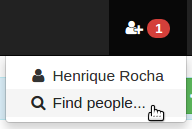
\includegraphics[width=\textwidth]{figures/test_ui_01.png}
        a) Friend list path
\label{fig:minipage1}
\end{minipage}
\begin{minipage}[b]{0.35\linewidth}
    \centering

    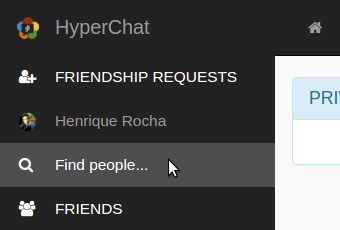
\includegraphics[width=\textwidth]{figures/test_ui_02.png}
         b) Friend requests path
\label{fig:minipage2}
\end{minipage}
\begin{minipage}[b]{0.2\linewidth}
    \centering

    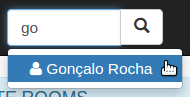
\includegraphics[width=\textwidth]{figures/test_ui_03.png}
         c) Search bar path
\label{fig:minipage2}
\end{minipage}

    \caption{Multiple paths for finding people}
    \label{fig:test_ui_01_02_03}
\end{figure}

On the second task one user clicked on the friends list for adding a friend to room and by consequence made him leave the conference room to the user profile. We solved this problem by showing a pop-up with the user profile and an additional button to add the user to the conference room as it can be seen on figure \ref{fig:test_ui_04}.

\begin{figure}[!htb]
\centering
\begin{minipage}[b]{0.7\linewidth}
\centering

    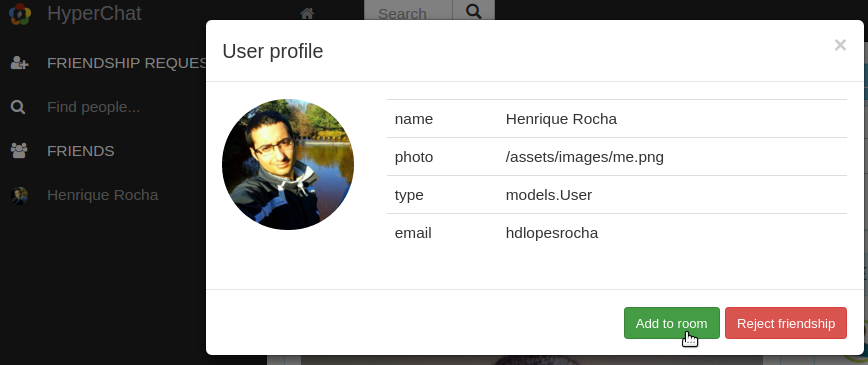
\includegraphics[width=\textwidth]{figures/test_ui_04.png}
\end{minipage}


    \caption{Adding user to conference room from user profile}
    \label{fig:test_ui_04}
\end{figure}

On the third task we noticed that both users were not expecting to search the content directly from the search bar, instead they used the time-line.

On the fourth task both users didn't placed their annotations on wright place, we only provide one way to place annotations, which is by dragging them on the time-line. 
After creating an annotation users also didn't understand that they had to save their changes on the time-line, we solved this problem by saving automatically each time the user changed any annotation, the old user interface can be seen on figure \ref{fig:test_ui_05}.

\begin{figure}[!htb]
\centering
\begin{minipage}[b]{0.3\linewidth}
\centering

    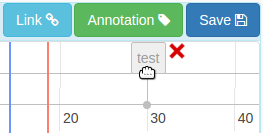
\includegraphics[width=\textwidth]{figures/test_ui_05.png}
\end{minipage}


    \caption{Save button that was removed}
    \label{fig:test_ui_05}
\end{figure}

Both users had success with fifth task but they revealed difficulties choosing the time interval for the hyper content, we are aware that this is a difficult task and that's why we have introduced the \emph{QR code} content creation mechanism which was very easy to learn.

We have also gathered comments and suggestions after letting the users explore our system, extra improvements were made such as:

\begin{itemize}
\item Giving feedback to user when saving content and collaborative editors.
\item Support file upload on our chat.
\item Starting with our time-line more zoomed in order to give more sensation of time.
\item Create content with starting time and duration instead ending time.
\end{itemize}

  \subsubsection {Second phase}